\section{DymelData}
\label{sec:DymelData}
\texttt{DymelData} ist eine Datenmenge, die mit dem \texttt{Recorder} (siehe Sektion \ref{sec:recorder}) erstellt wurde. Sie umfasst insgesamt 14410 Gesten in unterschiedlichen Konfigurationen. Ich habe diese Datenmenge
einerseits aufgenommen, um unter den in meinem Zimmer vorliegenden Lichtverhältnissen die Modelle miteinander vergleichen zu können und andererseits, um Test- und Trainingsdaten für NullGesten bereitzustellen. In den
bisherigen Datenmengen waren nur wenige Einträge mit NullGesten hinterlegt.
\subsection{Konfigurationen}
\subfigbox{
\subfigure[Geringe Helligkeit]{\label{subfig:light_low}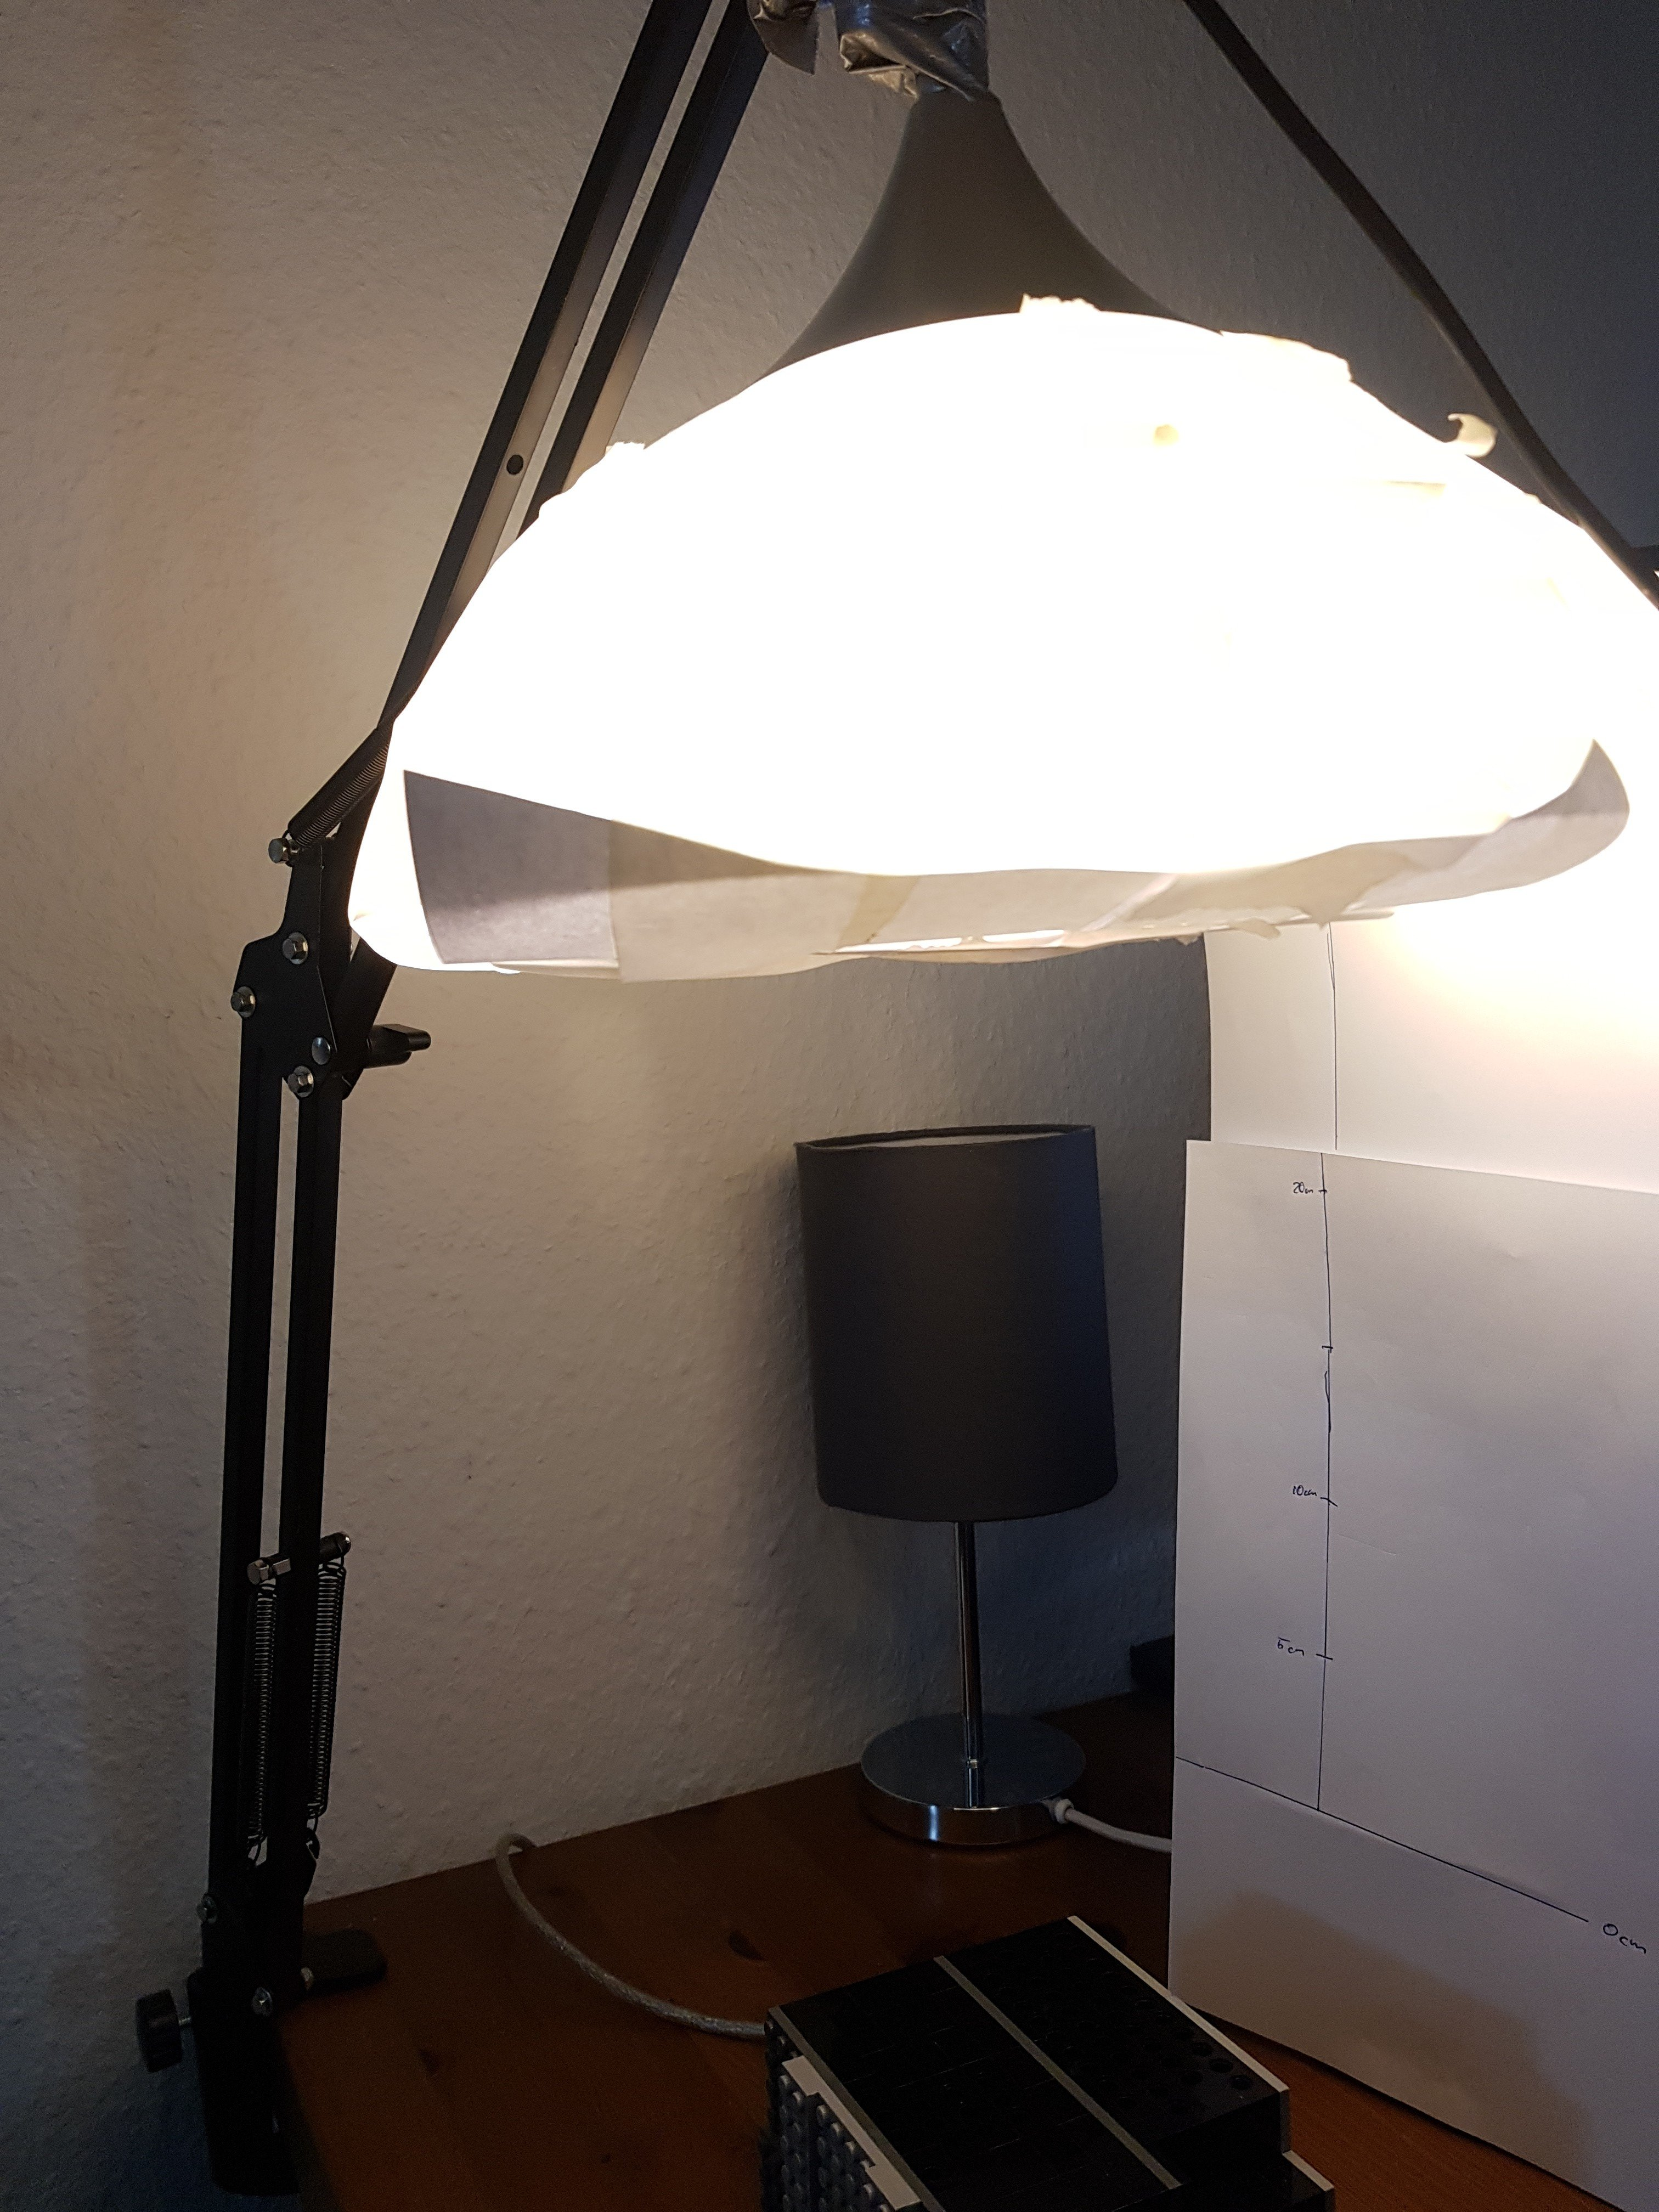
\includegraphics[width=0.33\linewidth]{images/light_low.jpeg}}\hfill%
\subfigure[Halbe Helligkeit]{\label{subfig:light_medium}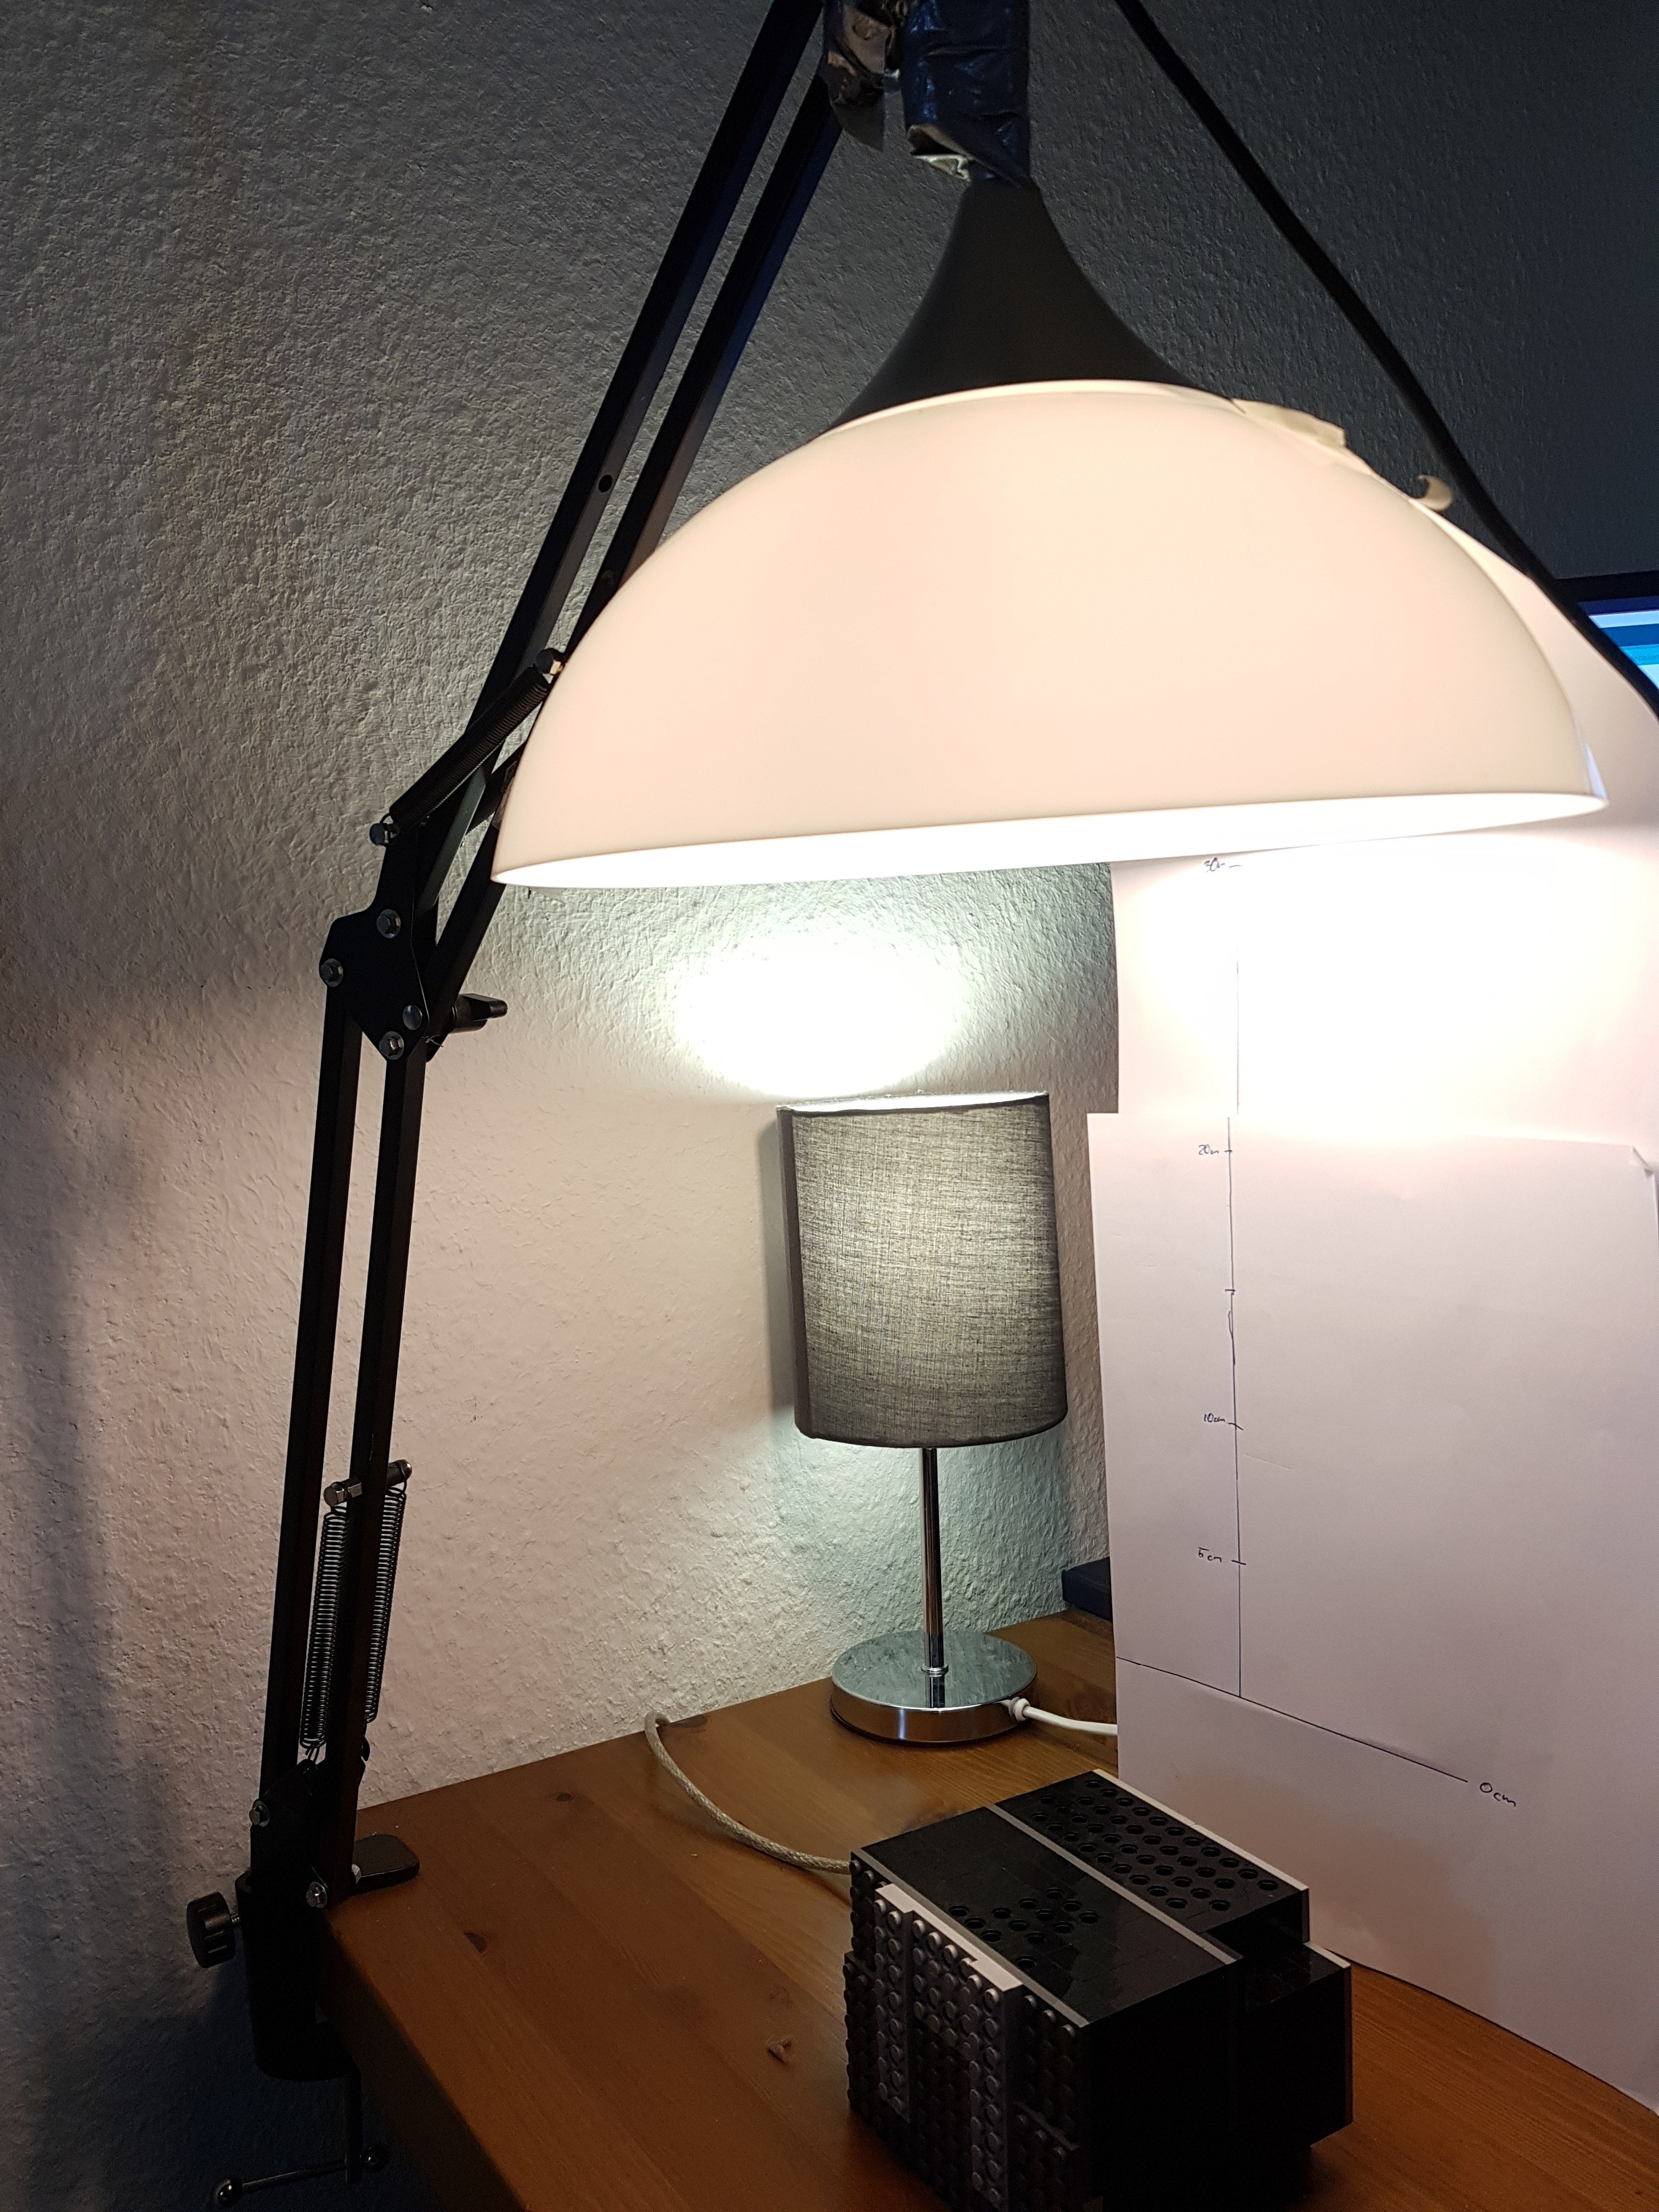
\includegraphics[width=0.33\linewidth]{images/light_medium.jpeg}}\hfill%
\subfigure[Hohe Helligkeit]{\label{subfig:light_high}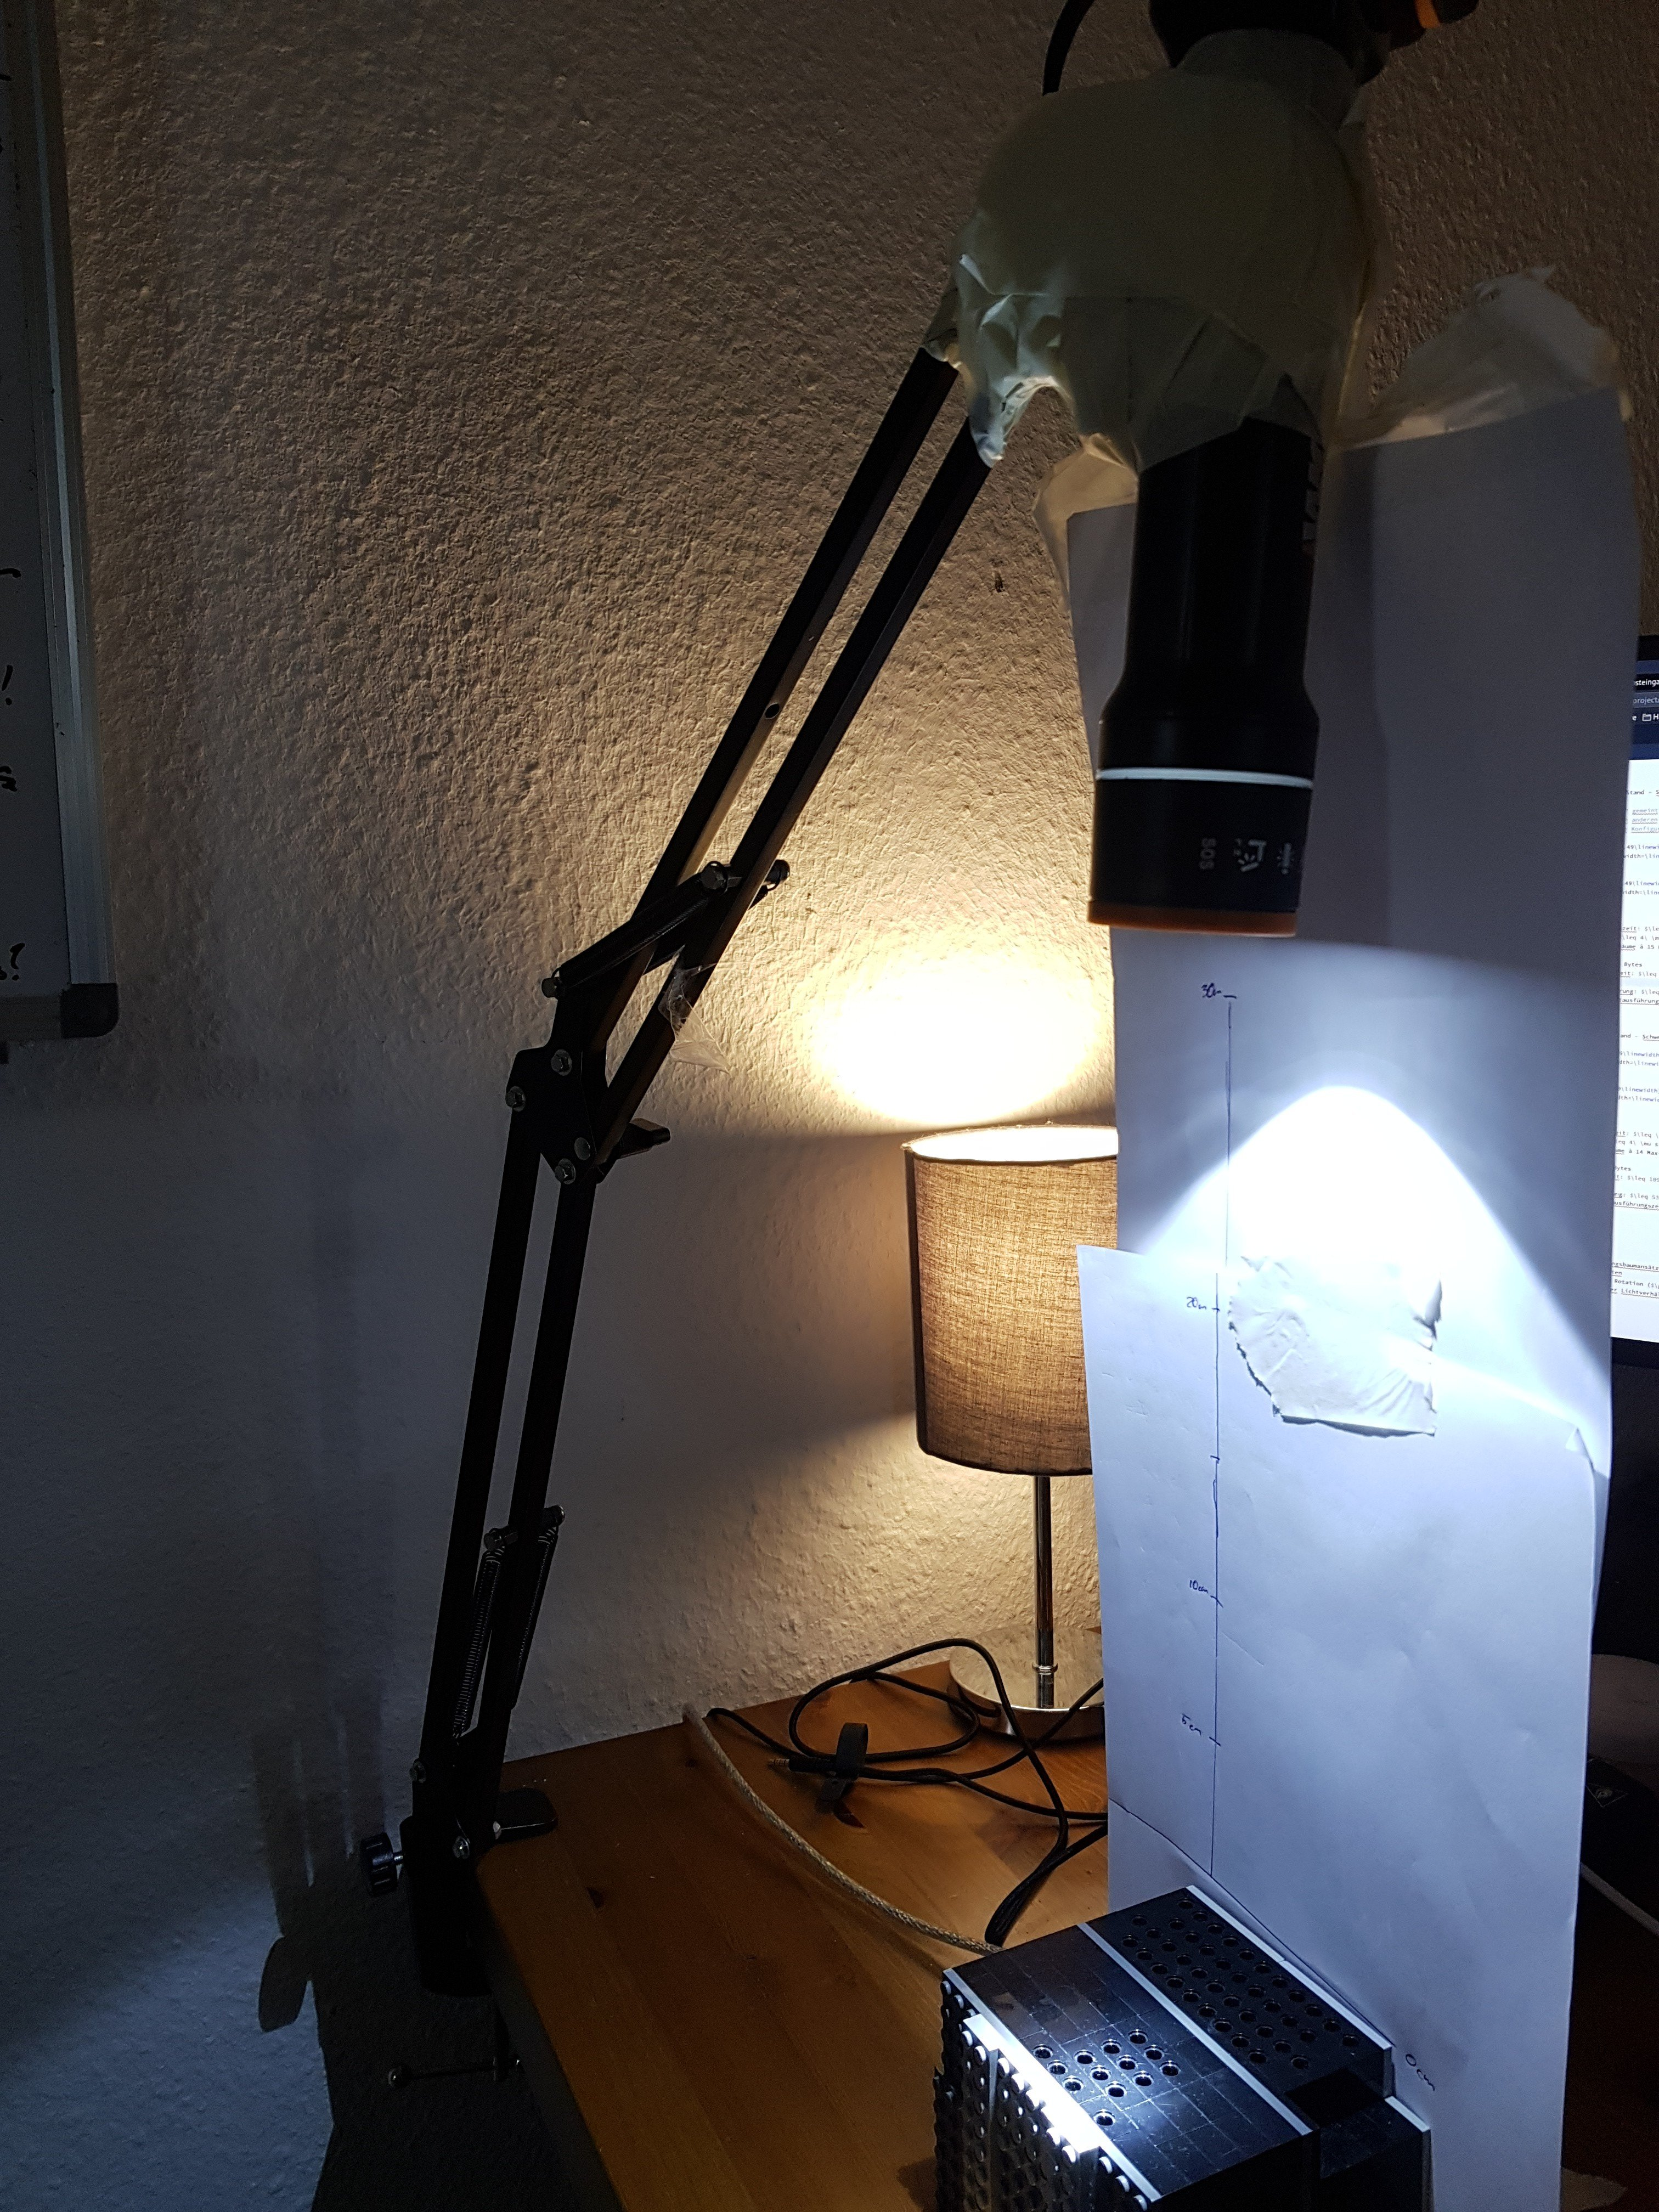
\includegraphics[width=0.33\linewidth]{images/light_high.jpeg}}%
}{Verschiedene Helligkeitsstufen unter denen die Gesten von \texttt{DymelData} aufgenommen wurden.}{fig:different_lights}
Jede Geste wurde unter jeder Konfiguration ca. 100 mal aufgenommen bei 90 Bildern pro Sekunde. Insgesamt wurden in 3 Lichtverhältnisse und 4 Distanzen, 6 verschiedene Gesten (Links nach Rechts, Rechts nach Links,
Oben nach Unten, Unten nach Oben und 2 NullGesten) jeweils schnell und langsam aufgenommen. Geringe Helligkeit war im Durchschnitt bei ca. 140, Halbe Helligkeit bei ca. 659, Hohe Helligkeit bei ca. 908. Alle waren
relativ gleichmäßig ausgeleuchtet. Der Unterschied liegt in der Art der Lichtquelle. Während bei den Lichtquellen \ref{subfig:light_low} und \ref{subfig:light_medium} relativ breit Licht gestreut hatten,
war \ref{subfig:light_high} eine Punktlichtquelle, wodurch besonders dort der Kontrast sehr stark ist. Die Gesten wurden in den Abständen 5 cm, 10 cm, 20 cm und 25 cm aufgenommen.
\subsection{NullGestures}
Explain what it is in general
\subsubsection{Corner}
\subsubsection{Same side in and out}
\subsubsection{Rotations}
\subsection{Synthetic Brightness Dataset}
